%!TEX root = ../main.tex
%=========================================================

\section{Ads placement}
\label{sec:placement}
In the following, we provide a description of distributing advertisement in the network and discuss the process of search and establishing sub-protocol connections. 


\subsection{Data Structures}
We start by describing data structures necessary for topic-specific registrations and lookups. 

\para{Registration Table}
In order to execute the ad distribution process described below,  each advertiser maintains a per-topic \emph{registration table} for each advertised topic. The table keeps track of the ongoing registration attempts with different registrars.  The registration table is similar to the routing table used in Kademlia protocol (as described in \Cref{sec:background}). It stores advertiser's peers divided into k-buckets. However, instead of placing nodes in buckets based on the distance from the advertiser, it uses the distance from the topic ID. I.e. the registration table stores $k$ potential registrars for every distance range (bucket) from the topic ID (\Cref{fig:ticket_table}). When created, the table is initialized with peers from the routing table. 

\dk{Imo, it is not clear if there is a single topic table each node maintains, or if each node has one topic table for each Topic ID. Especially because the previous Section said there is a \emph{second} table for topics.}

\begin{figure}
    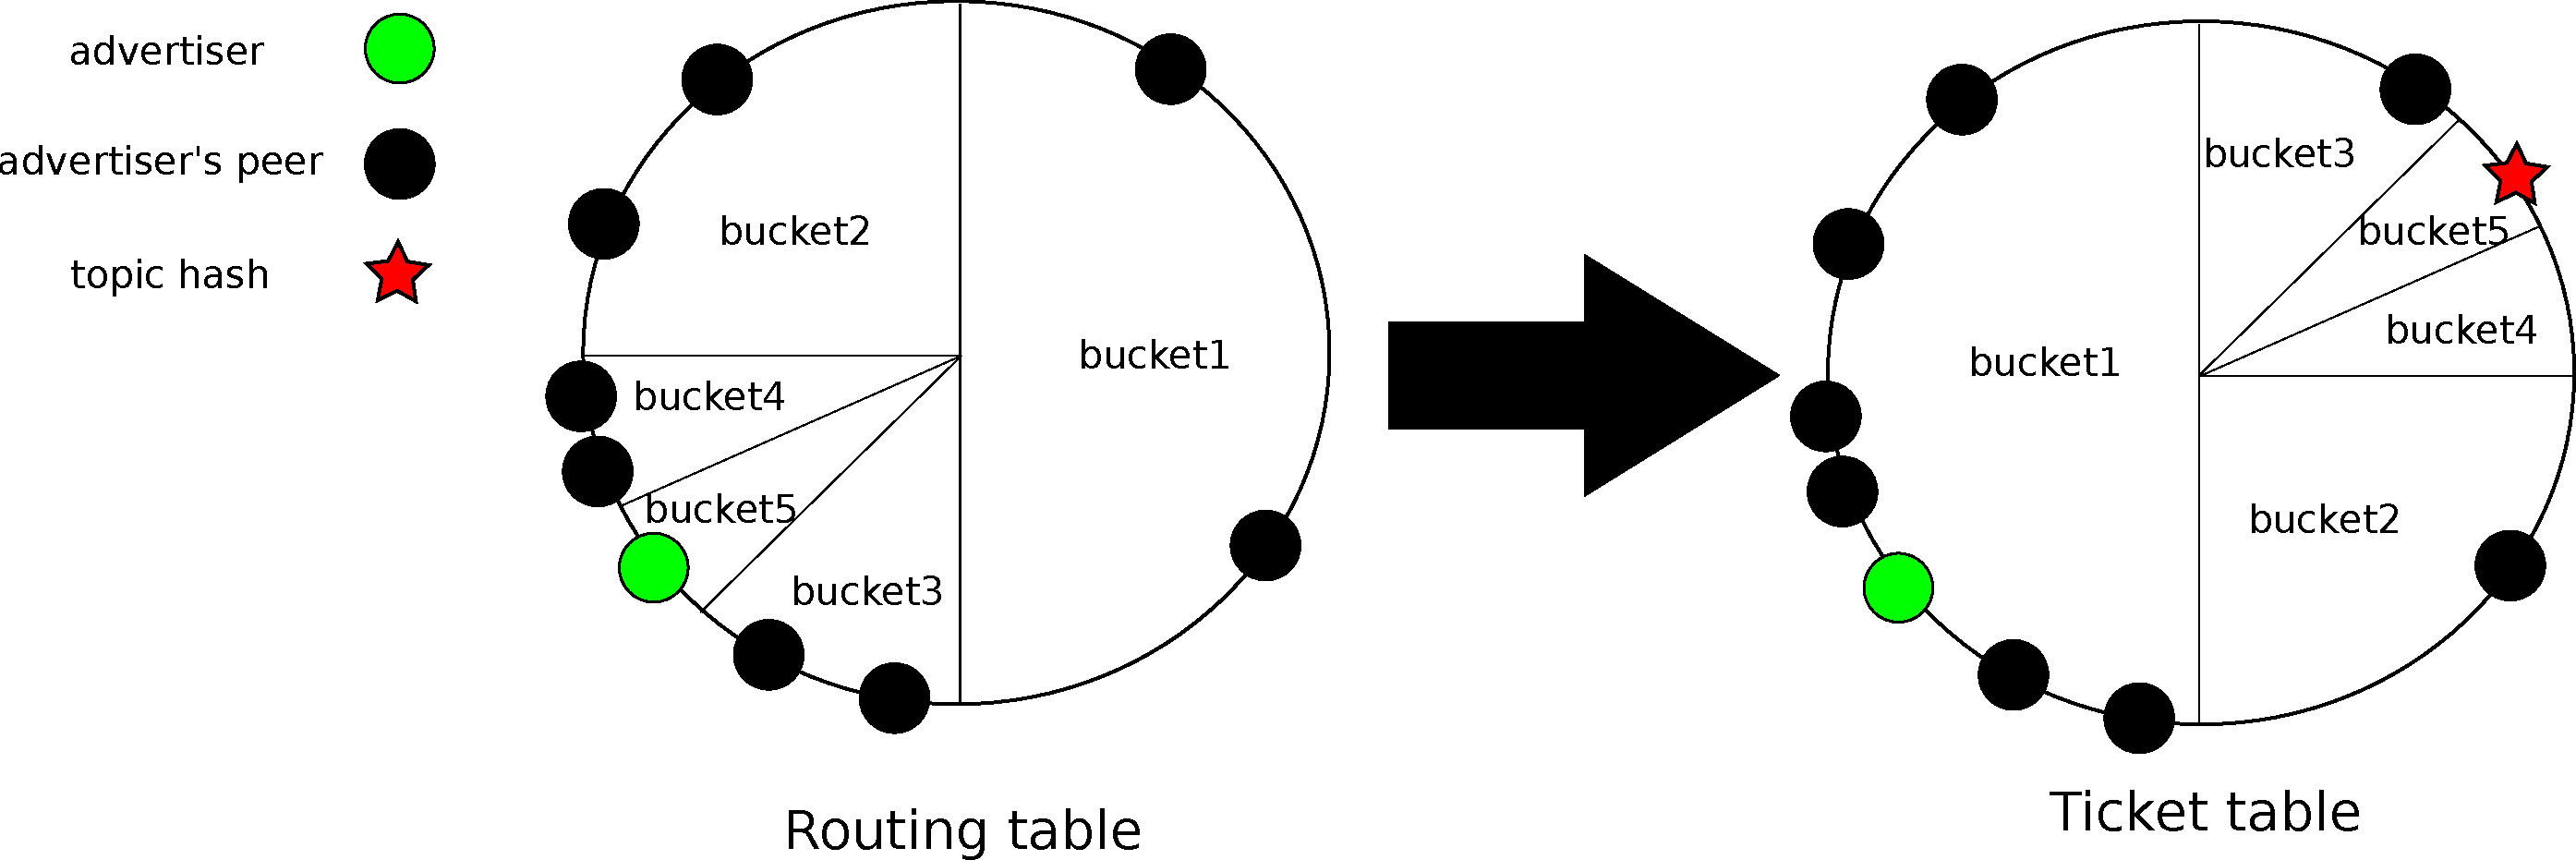
\includegraphics[width=0.45\textwidth]{img/ticket_table}
    \caption{Creation of ticket table from the routing table.}
    \label{fig:ticket_table}
 \end{figure}

\para{Search Table}
The ad lookup process is supported by a \emph{search table}. 
Searchers maintain a separate table per topic they are currently looking for. 
\ie for each topic the client wants to start discovering nodes, a new \emph{search table} is created. 
Similar to the \emph{registration table}, the \emph{search table} also stores k-buckets of registrar nodes by distance to the topic hash and buckets are initially filled from the local routing table organised by the distance from the topic hash.

%and a new 'search table' is created for each topic. 
%The bucket size \texttt{k}  of the search table should be relatively large in order to make the search efficient. 
%By default we use\texttt{k=16},  similarly to the local routing table (Kademlia DHT).
%Tickets are not required for search and nodes can not be added multiple times in the same k-bucket.

\subsection{Distributing ads across registrars}\label{sec:registration_multi}
When an advertiser wants to associate themselves with a topic, they start by creating a topic-specific \emph{registration table} (as described above). 
Every peer present in the registration table is a potential registrar. 
The objective of the ad placement process is to continuously maintain $K$ active (\ie unexpired) registrations in every bucket. 
Buckets located close to the topic hash cover less hash space than buckets located further away and, in turn, contain less potential registrars. 
Placing a fixed amount of ads per bucket, make registrars close to a topic hash more likely to receive registrations for that specific topic. 
Increasing $K$, makes the advertiser easier to find at the cost of increased communication overhead. 

The advertiser starts by the first bucket (the furthest away from the topic hash) in the \emph{registration table}, selects $K$ random peers and attempts to perform a registration. 
\dk{Why not all bucktes in parallel?}
We describe details on the registration procedure in \Cref{sec:registration}. 
A successful registration places an ad on an advertiser for a fixed amount of time $t_\textit{lifetime}$.
If a registration is unsuccessful (the selected registrar is down or refuses to store the ad), the advertiser selects another random peer from the same bucket and retries the registration process. 
The advertisers always maintains $K$ attempts and/or successful registrations per bucket unless less than $K$ peers are present in a specific bucket. 
The advertiser repeats the process for every bucket in the registration table. 
\michal{An algorithm here?}

As mentioned above, the \emph{routing table} is initialized with the peers already present in the routing table. It is thus possible that an advertiser will not know any nodes in buckets located close to the topic hash\footnote{This usually happens when the advertiser's ID is distant from the topic hash.}. 
To fill the empty buckets, the advertiser asks potential registrars to return $N$ closest peers to the topic hash they know of. 
The procedure is similar to the regular DHT \emph{FIND\_NODE} operation described in \Cref{sec:background}. 
The registrars respond with a list peers regardless of the success of the registration operation. 
The advertiser uses the returned information to populate its \emph{registration table}. 
As the advertiser progresses through the buckets, it queries potential registrars located closer to the topic hash and thus having a more detailed view of this part of the network. 
Similarly to the DHT routing, the registration procedure is guaranteed to find the closest node to the topic hash in the network. 
\ramin{Why not just use FIND\_NODE?}
\michal{It's basically FIND\_NODE but based on a different table (registration table, rather than the routing table) and performing the registration on top of traversing the DHT. IMO it's easier to have a seperate name here.}

%In addition to that, every time a node sends a ticket or registration request, the registrar replies with the closest nodes to 'the topic hash' that it knows. 
%This helps filling up k-buckets without sending additional lookups. 
%Also, when performing topic search (sending lookups for specific topics),  closest known nodes to 'the topic hash' are attached by the registrar node in the response.




\subsection{Lookup operation}\label{sec:lookup}
To find ads, \sysname uses a process similar to the registration procedure. 
The goal is to find $N_\textit{lookup}$ node advertised with a specific topic. 
The searcher starts by creating a topic-specific \emph{search table} initially populated with nodes from the \emph{routing table}. 
\michal{Should we have separate $K$ for registration and lookup? You might argue that if less ads are placed, more lookups are needed and vice-versa.}
\sergi{we actually use different values of $k$ for registration and search.  we could name it differently}
The searcher progressively moves through buckets (starting from the furthest away), randomly chooses $K$ registrars per buckets and sends them lookup requests. 
Each queried registrar responds with a list of $N_\textit{return}$ topic-specific advertisers the registrar know of. If the total number of topic-specific registrations is larger then $N_\textit{return}$, the registrar return a random subset. While both $N_\textit{return}$ and $N_\textit{lookup}$ are protocol parameters, the amount of ads returned by a single registrar must be lower than the total number of ads searchers are aiming to find $N_\textit{return} < N_\textit{lookup}$. It allows to diversify sources of ads received by the searcher. I.e., a single malicious registrar is not able to stop an honest searchers from contacting other nodes.
There is a tradeoff between overhead and security when choosing $N_\textit{return}$ and $N_\textit{lookup}$. 
By requiring a large amount of total ads to stop the search ($N_\textit{lookup}$) and low amount of ads returned by registrar $N_\textit{return}$ a higher diversity of data sources is achieved by the cost of contacting a large number of registrars. On the other hand, similar values of both $N_\textit{lookup}$ and $N_\textit{return}$ reduce the overhead but increase the danger of a searcher receiving ads uniquely from malicious nodes. Finally, low values of $N_\textit{lookup}$ stop the search operation early,  before reaching registrars close to the topic hash, contributing to more equal load spread. We investigate the impact of both parameters in \Cref{sec:eval}.
\ramin{In practice, is $N_\textit{lookup}$ a parameter that can be controlled? It sounds like something application-specific, e.g. for some applications, it might be enough for a searcher to just find one node to be able to use the application as intended. Search for 10 and choose one randomly from them?}
\michal{That's a good point. Not sure if we should allow the application to control both $N_\textit{lookup}$ and $N_\textit{return}$. Or maybe fix a ration between both and automatically set $N_\textit{return}$ once $N_\textit{lookup}$ is chosen by the application.}

Once ads are discovered,  the searcher can initiate topic-specific connections based on rules specified by the application. 
Applications do not only receive a list of potential nodes to connect but also the registrar node source of the search response.
In order to avoid eclipse attacks it is recommended not to start connections with nodes coming from the same registrar. 
Therefore connections are initiated always trying to keep the maximum diversity of the  registrars nodes used.
Once all nodes received have been used to try new connections,  a new search process is initiated. 

%\subsubsection{Updating connections}
%\michal{Didn't touch this subsection. Should it be here?}
%\sergi{i integrated some part in the last paragrah and the resti is already in the background section}
%Using the search results, a searcher updates its subprotocol-specific connections. 
%For instance,  each Ethereum client keeps connections towards 50 other nodes,  2/3 of those are for inbound connections (\ie 34 connections) where the client has no control over them, and the rest (about 16 connections) are four the outbound connections initiated towards the discovered nodes using the discovery protocol. 
%When a lookup is done,  the nodes discovered are stored in a buffer. 
%For each node of the buffer a connection is initiated. 
%The connection can be successful when the node targeted is alive and has empty slots in the inbound connections,  otherwise the connection is unsuccessful and a new node is selected.
%The nodes from the buffer are consumed as connections are attempted to the nodes.
%The buffer not only stores the nodes information but also the registrar node that replied with it.
%In order to avoid eclipse attacks it is recommended not to start connections with nodes coming from the same registrar. 
%Therefore connections are initiated always trying to keep the maximum diversity of the  registrars nodes used.

%\onur{need to explain this process since security depends on that.}

%All the modifiers from the first part of the equation increase with increasing number of the same items that are already in the table, i.e., reduction in diversity. Thus it's getting increasingly difficult to register ads for the same IP/ID/topic. For instance, ads for less popular topic will receive lower waiting times than popular ones. Note that the table does not prevent anyone from registering, but rather makes it slower for already popular items. Such a mechanism promotes diversity in the table and protects against Sybil attacks so that an attacker who is in control of a limited pool of IP addresses won't be able to dominate the table with many ads. The low exponent for the topics is motivated by the topics in the network that are likely to follow a skewed (e.g., a zipf-like) distribution. In contrast, honest nodes' IPs/IDs should follow a uniform distribution.

%The latter part of the formula is determined based on a multiple of ad-lifetime and the current utilisation (i.e., occupancy divided by capacity) of the table. When the utilisation becomes closer to 1.0, the base time becomes very large due to a very small denominator. Before the waiting time becomes infinite (when utilisation becomes 1), the waiting time becomes extremely high, in which case the advertisers give up as explained in the ad distribution process.

%The advertiser attempts to place an ad on each registrar and keeps the latest ticket issued by that registrar. It also keeps references to all pending tickets in a priority queue keyed by the expiry time of the ticket so it can efficiently access the next ticket for which a placement attempt is due.
%Since the table is limited to K values per bucket,  this means there are K on-going registrations per distance to the topic hash id. 
%The number of buckets used in the ticket table is a configurable parameter, but it is recommended to use small number of buckets,  instead of using a bucket per bit of the address space,  to avoid overloading registrars with IDs close to the topic hash. 
%Any node with a distance below the maximum distance minus the number of buckets will be stored in the same bucket.
%In our evaluation we used a ticket table with 10 buckets. 



%This objective is achieved by the advertisers setting a timer with a duration of ad-lifetime immediately upon the receipt of a REGCONFIRMATION from a node in a bucket b, and once the timer expires (after ad-lifetime passes) the advertiser starts a fresh registration with a node that is also located in bucket b. 
%The ticket table is used to store the tickets obtained for each on-going registrations and to keep track of the expiration times of active registrations.

%\subsubsection{Bucket refresh}

%The Ticket table needs to be initialised and refreshed to fill up all the per-distance k-buckets. 
%Ideally,  all k-buckets should be constantly full,  meaning that the advertisers place registrations at registrars in all distances to the topic hash. 
%An option to fill up all k-buckets would be to send periodic lookups for the specific distance to the topic hash, but since there are some distances that tend to be empty in the id space,  sending periodic lookups for the topic hash may create an additional overhead that can be too expensive and create too much traffic in the network. To avoid that, initially, the 'ticket table' k-buckets are filled performing local Ethereum routing table lookups to all distances to the 'topic hash' of the advertised topic.


%\michal{The below seems like an implementation detail.}
%There is  also a refresh bucket process,  similar to the Kademlia DHT table,  where periodically a random bucket is checked to see if it is empty.
%The \texttt{refresh time} is a configurable parameter. 
%We set a \texttt{refresh time=10 seconds} as a reference for our performance evaluation.
%During the refresh process,  in case the bucket checked is empty, 
%a local lookup to the Kademlia DHT table is performed. 
%In case no nodes have been found for the bucket distance,  a Kademlia lookup is performed towards the topic hash~\footnote{The lookup is performed by sending a FINDNODE message,  as described inhttps://github.com/ethereum/devp2p/blob/master/discv4.md.}
%Also, all nodes in the checked bucket are pinged to check they are still alive. 
%In case they are not, tickets for those dead nodes are removed from the ticket table and registrations to new nodes are initiated.




%We implemented and evaluated a lookup strategy that choose which nodes from which buckets ask first trying to diversify the nodes discovered as much as possible and trying not to overload nodes close the topic hash.
%A random node is picked from a bucket following a round-robin approach. 
%It starts picking a random node from the highest distance bucket and follows to the next distance in the bucket list.
%In order to find new results,  bucket entries are replaced when the node fails to answer or when it answers with an empty list of ads. 

%There is also a refresh process,  equivalent to the \emph{ticket table} refresh process, where random buckets are selected and all nodes in the buckets are checked for liveness.
%In case the bucket is empty a Kademlia lookup is performed towards the topic hash.
